\subsection{Time series of the factor scores and exceedance}\label{sec:serie-tiempo}

The response \texttt{excede\_anio\_5} (\cref{sec:obj:objetivo}) and the
three factor scores of \cref{sec:analisis-factorial} are characterized here
over time: their origin and validity, already established, are not
revisited, only their behavior as series.

\subsubsection{From station-day to metropolitan area}

Any time-series decomposition requires a series without gaps, and the
station-day panel is not one. Only 2 of the 15 stations (\texttt{CE},
\texttt{SE3}) exceed 85\,\% coverage of valid station-days over the
2021--2025 calendar, and the worst, \texttt{NO3}, reaches 25\,\%; overall
coverage is 68.0\,\%. Filtering to the best-covered stations does not solve
the problem, it hides it in the three that survive the cut.

The alternative is to aggregate the 15 stations into a daily
metropolitan-area value, which is only reasonable if stations are not
independent of one another on the same day. The cross-sectional correlation
(Pearson, station against station, same day) ranges from a mean of 0.50 for
ventilation to 0.85 for photochemical forcing, with a barely negative
minimum only for ventilation. This is consistent with the physics:
temperature and solar radiation are regional-scale phenomena, whereas wind
depends on the local topography of the valley. This correlation is also the
largest violation of independence in the dataset, relevant to any model that
treats each station-day row as an observation ---including the
autocorrelation limitation already declared in
\cref{sec:limitaciones-clasificacion}.

Given the insufficient coverage per station and the high cross-sectional
correlation, the data are aggregated at the metropolitan-area level by
averaging the stations that report each day. The average recovers
99.94\,\% coverage of the daily calendar; a single day, 2021-02-16, has no
station at all and is imputed by linear interpolation ---only because the
MSTL decomposition requires a series without gaps, not because the gap
ceases to exist.

\subsubsection{MSTL decomposition}

MSTL is fitted with weekly (7) and annual (365, not 365.25: MSTL requires
integer periods and the accumulated drift over 5 years is about one day,
negligible) periods to the four metropolitan-area series. The weekly cycle is
strongest for primary combustion ---the weekday/weekend pattern of traffic
and industrial activity--- and weakest for the fraction of stations above the
threshold, which dilutes that pattern because it depends on several factors
at once.

\subsubsection{Residual autocorrelation}

The Ljung-Box test at lags 7, 14 and 30 rejects with $p<0.001$ for all four
series, in both versions (raw and MSTL residual) ---the same problem that
\cref{sec:analisis-factorial} noted for Bartlett: with $n=1{,}826$ daily
observations, the statistic grows with $n$ and rejects any non-trivial
autocorrelation, including that of the residual, where seasonality has
already been removed. The test does not discriminate; the magnitude of the
ACF does (\cref{fig:acf-excedencia}).

\begin{figure}[t]
  \centering
  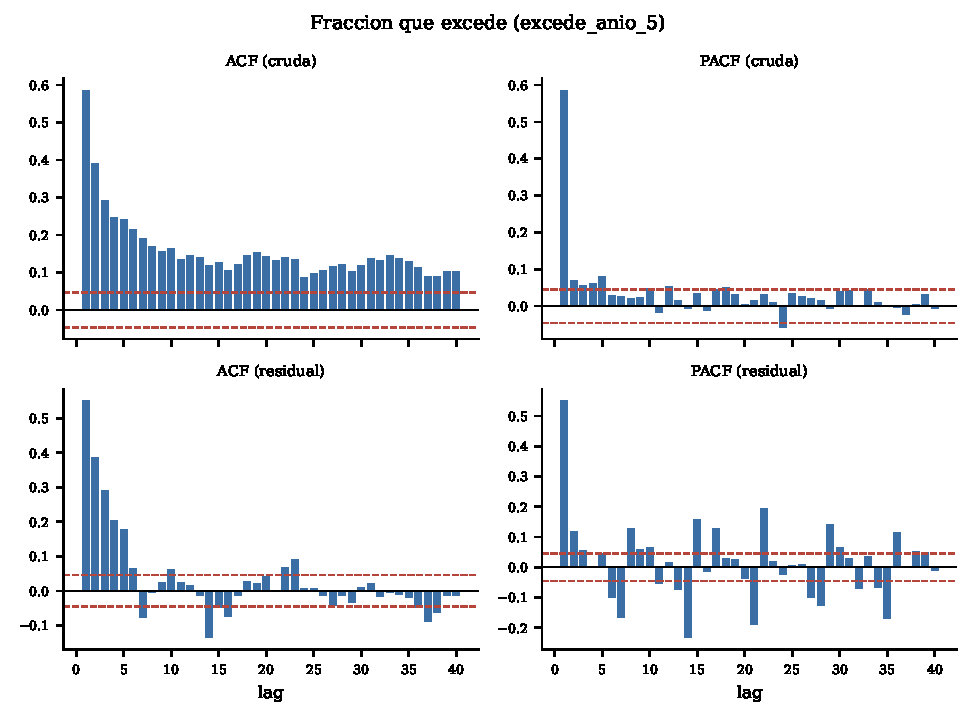
\includegraphics[width=\linewidth]{acf_pacf_frac_excede_anio_5.pdf}
  \caption{ACF and PACF up to lag 40 of the exceeding fraction: raw series
    (top) versus MSTL decomposition residual (bottom), with
    $\pm 1.96/\sqrt{n}$ band.}
  \label{fig:acf-excedencia}
\end{figure}

After MSTL, the lag-7 autocorrelation falls from 0.19--0.45 to values between
$-0.15$ and 0.05 in the four series ---the weekly seasonality practically
disappears. The lag-1 autocorrelation, by contrast, remains between 0.49 and
0.71 in the residual of all four series. That day-to-day persistence is not
seasonality: it is genuine short-term autocorrelation, which MSTL is not
designed to remove. It quantifies, with a continuous series without gaps, the
same temporal dependence that \cref{sec:limitaciones-clasificacion} identified
as the reason the standard errors of the logistic model are optimistic.

Two consequences carry over to the autoregressive model of
\cref{sec:autorregresivo}: lags must be computed on the metropolitan-area
series reindexed to a regular daily calendar, never on the station-day
table, where the previous row may be a week away; and the day-to-day
dependence is genuine, not an artifact of seasonality, so a model that
ignores it leaves structure in the residuals.
